
\begin{frame}[ctb!]
\framtitle{GDSM Model Advective Diffusive Sensitivity}
For vertical advective velocities 
$6.31\times10^{-6}[m/yr]$ and above, lower reference diffusivities are 
ineffective at attenuating the mean of the peak doses for soluble, non-sorbing 
elements. 

\begin{figure}[htp!]
\begin{minipage}[b]{0.45\linewidth}
\centering
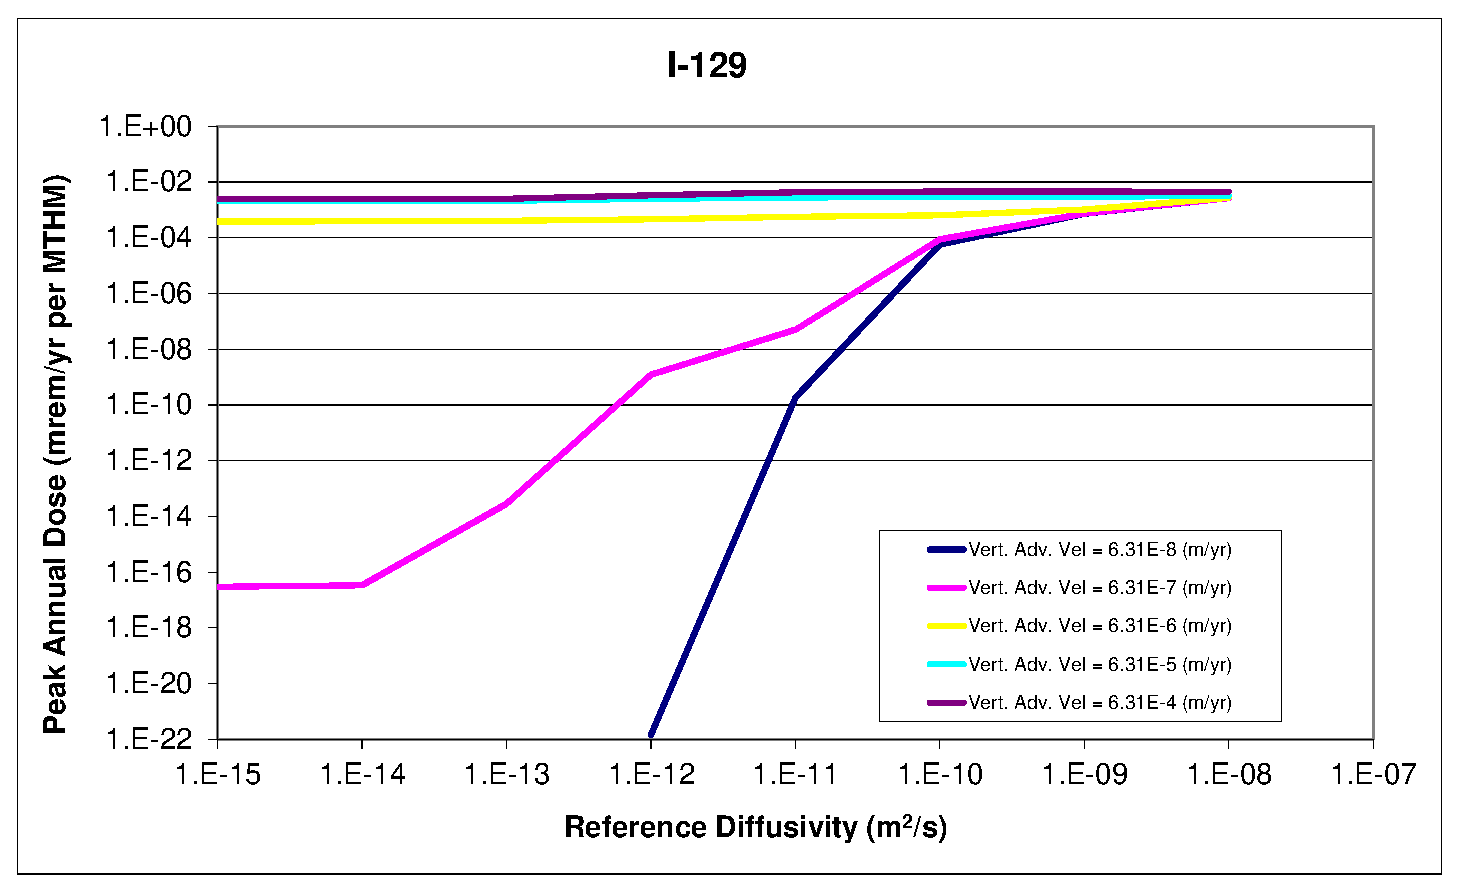
\includegraphics[width=\linewidth]{./nuclide_demonstration/I-129.eps}
\caption{$^{129}I$ reference diffusivity sensitivity.}
\label{fig:VAdvVelI129}

\end{minipage}
\hspace{0.05\linewidth}
\begin{minipage}[b]{0.45\linewidth}

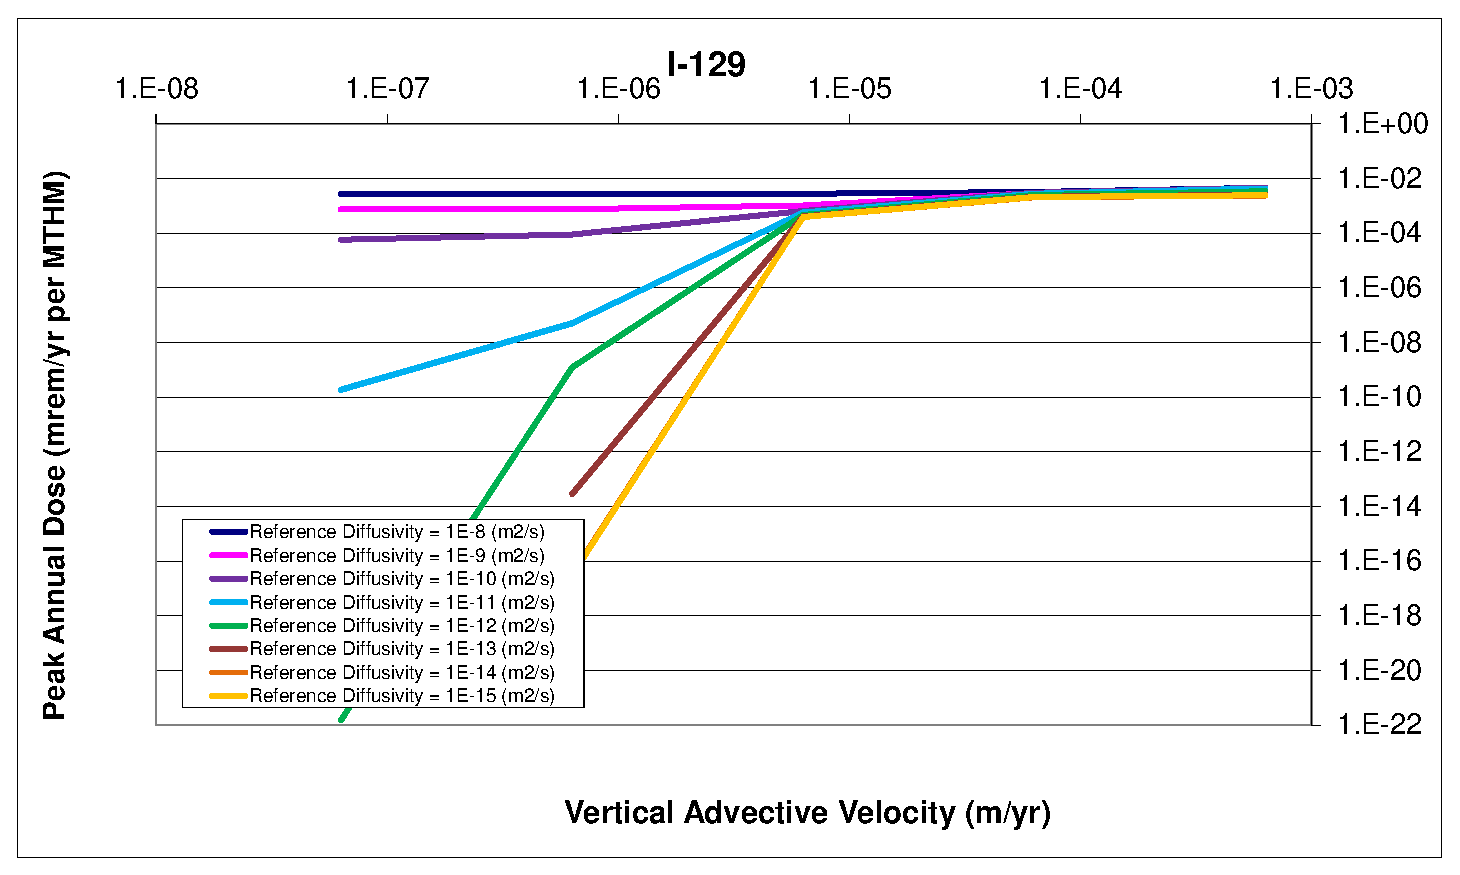
\includegraphics[width=\linewidth]{./nuclide_demonstration/I-129-VAdvVel.eps}
\caption{$^{129}I$ vertical advective velocity sensitivity.}
\label{fig:VAdvVelI129VAdvVel}

\end{minipage}
\end{figure}
\end{frame}
%\begin{figure}[htp!]
%\begin{minipage}[b]{0.45\linewidth}

%\includegraphics[width=\textwidth]{./nuclide_demonstration/Cl-36.eps}
%\caption{$^{36}Cl$ reference diffusivity sensitivity.}
%\label{fig:VAdvVelCl36}
%
%\end{minipage}
%\hspace{0.05\linewidth}
%\begin{minipage}[b]{0.45\linewidth}
%
%\includegraphics[width=\textwidth]{./nuclide_demonstration/Cl-36-VAdvVel.eps}
%\caption{$^{36}Cl$ vertical advective velocity sensitivity.}
%\label{fig:VAdvVelCl36VAdvVel}
%\end{minipage}
%\end{figure}

